% 2006 天津理科 Q19；固定候选 PDF 第 2 页（印刷页 337）。
% A,B,C,D 为矩形 ABCD 的顶点，O 为其对角线交点；CDE 为等边面。
% E,F 位于底面 ABCD 同侧。实线/虚线依印刷图可见关系重绘；底面对角线未补画。
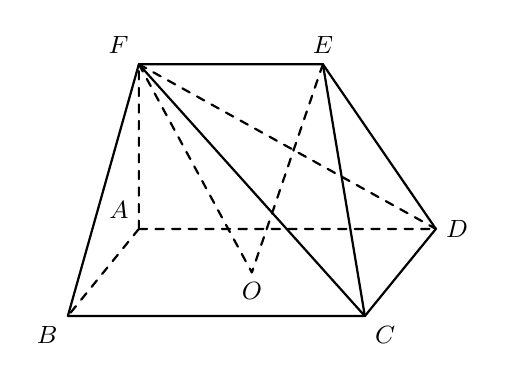
\begin{tikzpicture}[x=0.82cm,y=0.82cm,line cap=round,line join=round,line width=0.8pt,font=\small]
  \coordinate (A) at (1.1,1.35);
  \coordinate (B) at (0,0);
  \coordinate (C) at (4.6,0);
  \coordinate (D) at (5.7,1.35);
  \coordinate (O) at (2.85,0.675);
  \coordinate (F) at (1.1,3.9);
  \coordinate (E) at (3.95,3.9);
  % 底面遮挡边与图中虚线空间连线
  \draw[dashed] (A)--(B) (A)--(D) (A)--(F);
  \draw[dashed] (F)--(O) (E)--(O) (F)--(D);
  % 可见棱及内部实线
  \draw (B)--(C)--(D)--(E)--(F)--(B);
  \draw (E)--(C) (F)--(C);
  \node[above left] at (A) {$A$};
  \node[below left] at (B) {$B$};
  \node[below right] at (C) {$C$};
  \node[right] at (D) {$D$};
  \node[above] at (E) {$E$};
  \node[above left] at (F) {$F$};
  \node[below] at (O) {$O$};
\end{tikzpicture}
